\chapter{Introduction}
\clearpage

\section{What Is Data Mining?}
	
	{\bf Data mining:} is the process of automatically discovering useful information
	in large data repositories. Data mining techniques are deployed to scour large 
	databases in order to find novel and useful {\bf patterns} that might otherwise remain 
	unknown. They also predict capabilities to {\bf predict} the outcome of a future 
	observation.

	\begin{table}[H]
	\begin{tabular}{| p{6cm} | p{6cm} |}
		\hline
		{\bf What is data mining?} & {\bf What is not data mining?} \\ \hline
		"People that buys beer often buys potato chips", 
		grouping of documents by context & 
		lookup in catalog, normal search, information retrieval in general, etc \\ \hline
	\end{tabular}
	\end{table}	

	{\bf Knowledge Discovery in Databases (KDD): } is the overall process of converting raw 
	data into useful information. 

	The process of knowledge discovery in databases (from the book):
	\begin{enumerate}
		\item {\bf Preprocessing:} the input data can be stored in a varity of formats (flat files, spreadsheets, relational tables,etc). The purpose of preprocessing is to transform the input data into an appropriate format for the subsequent analysis. The steps involved in data preprocessing include fusing data from multiple sources, cleaning data to remove noise and duplicate observations, and selecting records and features that are relevant to the data mining task at hand. 
		\item {\bf Data Mining}
		\item {\bf Postprocessing}
	\end{enumerate}

		\begin{figure}[H]
			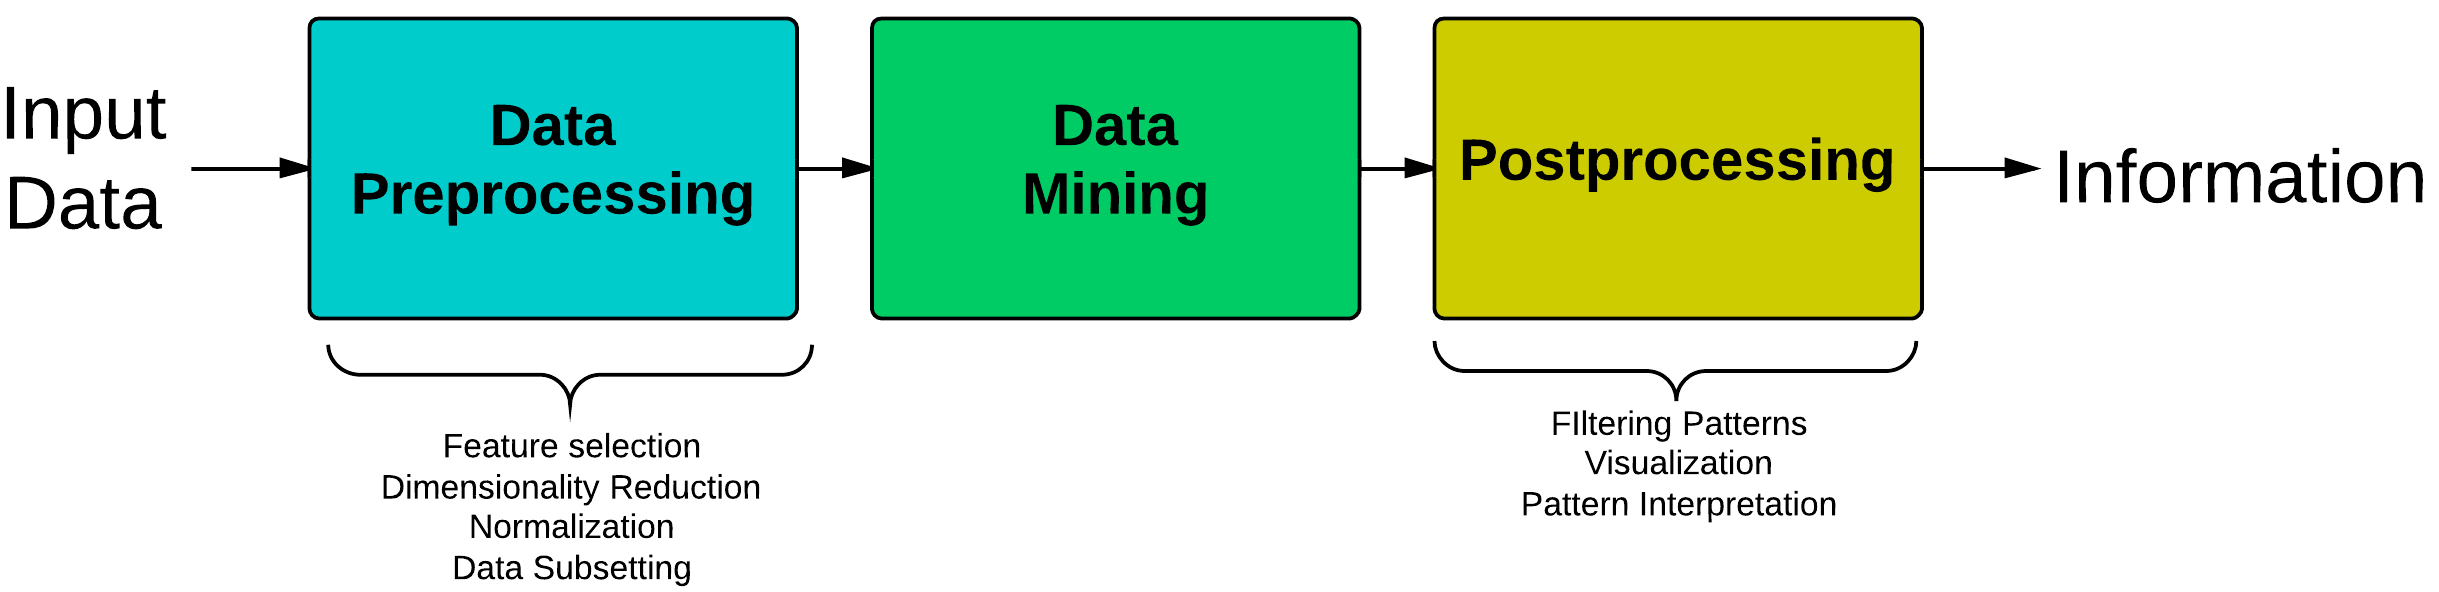
\includegraphics[width=\textwidth]{pics/KDD.png}
		\end{figure}

	\clearpage
	%http://dataminingwarehousing.blogspot.no/2008/10/data-mining-steps-of-data-mining.html
	The process of knowledge discovery in databases (blogpost)
		
	\begin{enumerate}
		\item {\bf Data Integration:} First of all the data are collected and integrated from all the 
		different sources.
		\item {\bf Data Selection:} We may not all the data we have collected in the first step. So in this 
		step we select only those data which we think useful for data mining.
		\item {\bf Data Cleaning:} The data we have collected are not clean and may contain errors, missing values,
		noisy or inconsistent data. So we need to apply different techniques to get rid of such anomalies.
		\item {\bf Data Transformation:} The data even after cleaning are not ready for mining as we need to 
		transform them into forms appropriate for mining. The techniques used to accomplish this are smoothing,
		aggregation, normalization etc.
		\item {\bf Data Mining:} Now we are ready to apply data mining techniques on the data to discover the 
		interesting patterns. Techniques like clustering and association analysis are among the many different
		techniques used for data mining.
		\item {\bf Pattern Evaluation and Knowledge Presentation:} This step involves visualization, 
		transformation, removing redundant patterns etc from the patterns we generated.
		\item {\bf Decisions / Use of Discovered Knowledge:} This step helps user to make use of the knowledge acquired to take better decisions.
	\end{enumerate}

		\begin{figure}[H]
			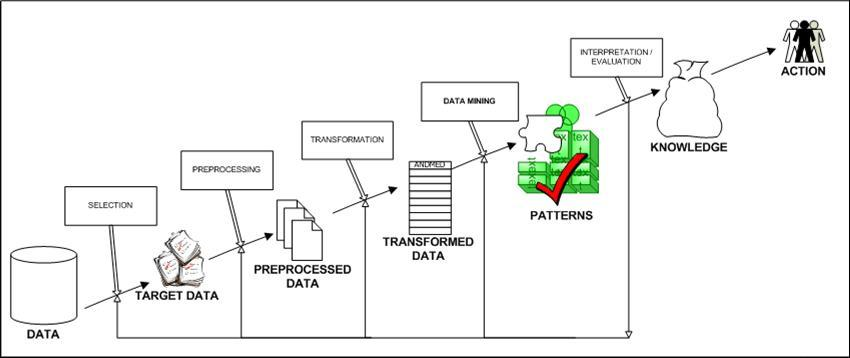
\includegraphics[width=\textwidth]{pics/datamining.jpg}
		\end{figure}

\section{Motivating Challenges}

	\begin{itemize}
		\item {\bf Scalability:} the massive explosion of saved data are becoming common. If data mining 
		algorithms are to handle these massive data sets, then they must be scalable.
		\item {\bf High Dimensionality:} It is now common to encounter data sets with hundres or thousands 
		of attributes instead of the handful common a few decades ago. This affects the algorithms used 
		because of the computational complexity increase rapidly as the dimensionality (thw number of 
		features) increases.
		\item {\bf Heterogeneous and Complex Data:} Data is often in a different format and contain different
		information. This makes it difficult to preprocess and analyse the data. The data that is collected is
		often very complex in terms of location, format, content and size. 
		\item {\bf Data Ownership and Distribution:} sometimes, the data needed for an analysis is not 
		stored in one location or owned by one organization. Instead, the data is geographically distributed 
		among resources belonging to multiple entities. This requires the development of distributed
		data mining techniques. 
		\item {\bf Non-traditional Analysis:} 
	\end{itemize}

\clearpage
\section{The Origins of Data Mining}

	Data mining as a confluence of many disciplines:

	\begin{figure}[H]
		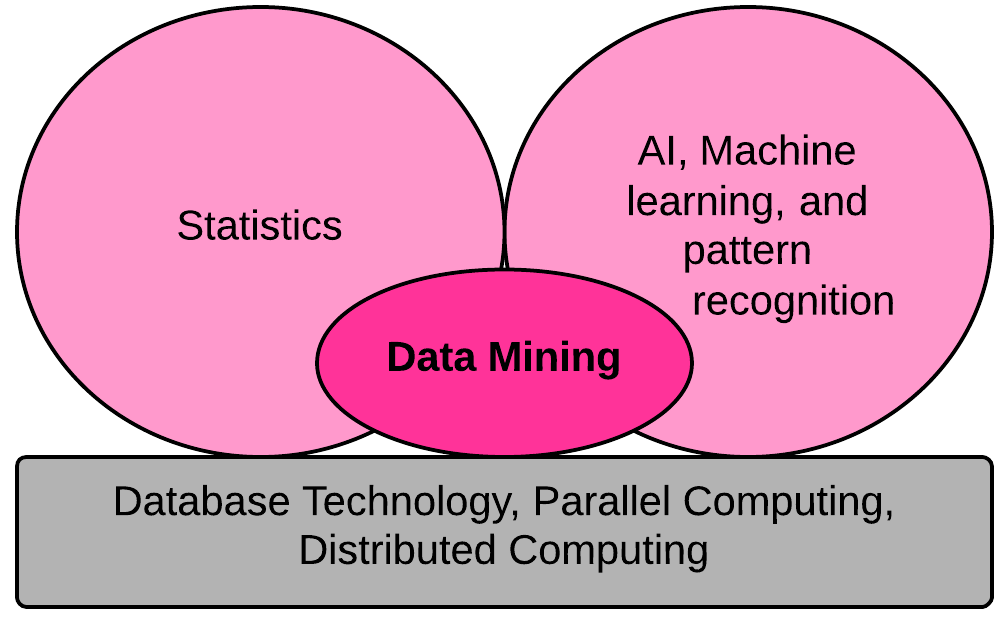
\includegraphics[scale=0.3]{pics/disciplinesDataMining.png}
	\end{figure}

\section{Data Mining Tasks}
	
	Data mining tasks are generally divided into:

	{\bf Descriptive tasks:} The objective of these tasks is to predict the value of a particular 
	attribute based on the values of other attributes. The attribute to be predicted is commonly 
	known as the {\bf target} or {\bf dependent variable}, while the attributes used for making the
	prediction are known as the {\bf explanatoy} or {\bf independent variables}. 

	{\bf Predictive tasks:} Here, the objective is to derive patterns (correlations, trends, custers, 
	trajectories, and anomalies) that summarize the undelying relationships in data. Descriptive 
	data mining tasks are often exploratory in nature and frequently require postprocessing tecniques
	to validate and explain the results. 

	{\bf The core data mining tasks:}
	\begin{itemize}
		\item {\bf Cluster Analysis:} seeks to find groups of closely related observations
		so that observations that belong to the same cluster are more similar to each other
		than observarions that belong to other clusters.
		\item {\bf Predictive Modeling:} refers to the task of building a model for the 
		target variable as a function of the explanatory variables. There are two types of 
		predictive modeling tasks: {\bf classification}, which is used for descrete target 
		variables, and {\bf regression}, which is used for continuous target variables. 
		\item {\bf Anomaly detection:} is the task of identifying observations whose 
		characteristics are significantly different from the rest of the data. Such observations
		are known as {\bf anomalies} or {\bf outliners}.
		\item {\bf Association Analysis:} is used to discover patterns that describe strongly
		associated features in the data. The discovered patterns are typically represented in the 
		form of implication rules or feature subsets. 

	\end{itemize}



